
%(BEGIN_QUESTION)
% Copyright 2006, Tony R. Kuphaldt, released under the Creative Commons Attribution License (v 1.0)
% This means you may do almost anything with this work of mine, so long as you give me proper credit

Shown here is a ``cut-away'' diagram of a simple pressure repeater, a device used to duplicate the pressure inside an enclosed process vessel with clean pneumatic (air) pressure, so it may be read with a remote gauge:

$$\includegraphics[width=15.5cm]{i00199x01.eps}$$

Describe the response of this device, step by step, to an increase in process pressure.  Hint: the diaphragm in this device is ``slack,'' meaning it has negligible spring effect.  This means even very small pressure differences are sufficient to move the diaphragm significantly.

Also, explain where we might want to use such a device, in lieu of simply connecting the pressure indicating gauge directly to the process vessel.

\underbar{file i00199}
%(END_QUESTION)





%(BEGIN_ANSWER)

As process pressure increases, the force pressing right on the diaphragm increases as well.  This makes the diaphragm move closer to the nozzle, making it more restrictive to air flow:

$$\includegraphics[width=15.5cm]{i00199x02.eps}$$

As air flow through the nozzle reduces, the ``backpressure'' built up by supply air through coming through the orifice increases.  This increased backpressure forces the diaphragm to the left, against the process pressure, until the diaphragm begins to back away from the nozzle and a new point of balance (equilibrium) is reached:

$$\includegraphics[width=15.5cm]{i00199x03.eps}$$

Because both pressures (process fluid, and air backpressure) act against the same amount of surface area on the diaphragm, the point of force balance between them will be when the two pressures are equal to each other.  Thus, the output air pressure (sensed by some remote pressure-measuring instrument) mirrors, or ``repeats,'' the process pressure.

\vskip 10pt

Applications for a pressure repeater are found in the biopharmaceutical and food processing industries.  If a pressure gauge were connected directly to the process vessel, the impulse tube connecting the gauge to the vessel would inevitably retain some of the process fluid.  In biopharmaceutical and food processes, bacteria will grow in stagnant process fluid, meaning that such lengths of tubing will act as reservoirs of harmful bacteria which may contaminate subsequent batches within the vessel.

The flush-mounted diaphragm of a pressure repeater is easily cleaned by ``clean-in-place'' (CIP) protocols used to clean the process vessel.  There are no crevices or small chambers for fluid to lie stagnant on the process side of a pressure repeater, therefore pressure repeaters eliminate the problem of bacterial contamination.

%(END_ANSWER)





%(BEGIN_NOTES)

The pneumatic repeater is one of the simplest examples of a force-balance instrument in existence.  Once students grasp the basic idea of how negative feedback works in a pneumatic system, they are prepared to understand more complex force- and moment-balance pneumatic mechanisms.

A good follow-up question to ask of your students after they understand the basic operation of a pressure repeater is what the supply air pressure must be for successful operation.  This question is closely related to the question of how much power supply voltage is needed to power an op-amp used as a voltage follower for a known signal level.  In both cases, obviously, the supply must be slightly greater than the highest input to be measured.

\vskip 10pt

For a practical example of a pneumatic pressure repeater, research the Foxboro/Eckhart model 139PP.

%INDEX% Measurement, pressure: pneumatic repeater

%(END_NOTES)


